\documentclass[]{article}
\usepackage{tikz}
\usepackage{listings}
\usepackage{scrextend}
\usepackage{textpos}


%opening
\title{A Theory of Micro Economic Behavior}
\author{``The first draft of anything is shit."}


\begin{document}

\maketitle
\newpage

%\begin{abstract}
%\end{abstract}



\subsection{Context}

There pretext of this document is as  follows. Human behavior as well as economics is difficult to predict due to factors such as scale, human variability in physical terms as well as the subjective nature of each individual. However at scale a model that can predict behavior of the average individual is sufficient to use. The goal being that this could be used to understand and optimize one's own situation as well as attempt to forecast the short term future.

\subsection{Assertions}

The theory rests on the bases if these assertions;
\begin{enumerate}
  \item \textbf{\textit{That effort can be defined in this context as the the total integration of pain/pleasure that the subject experiences over a duration of time.}}
  \item \textbf{\textit{That when a subject is presented with an opportunity of voluntary exchange that they will choose the option that minimizes their own net effort.}}
\end{enumerate}

However since each person has different predispositions to what activities they like or don't like the amount of effort that should be attributed to that activity differs person to person. Since subjects are all unique it would be inappropriate make value proportional to simply the net effort associated with a good or service, as tempting as \textit{that} may be. Instead metrics of effort can only be used for comparing the same subject. Also since some people have higher ambition, willing to expend more effort in the pursuit of return of effort, subjects have variability along this dimension.

Using these assumptions a basic model can be constructed from low level ideas. For instance; say two people living in a house both must do dishes and vacuum clean the carpet at some some point. Perhaps they roster this so that each person dose these jobs or do pitch in when necessary. If subject one dose not enjoy one of these jobs more than the other and, as it happens subject two, may also dislike the other job more, it this case there may be mutual benefit in each person doing all of one of the jobs. So long as from each person's perspective the trade is wanted, the amount of discomfort that each person experiences is reduced in comparison to the alternative over the duration of time. In this case there exists mutual benefit both parties that can be understood by the reduction of both parties 'effort'. A more rigid definition and explanation of effort will be addressed in a latter chapter. It is also worth pointing out that there may be an inequality in the effort saved for the parties. 


\subsection{Definition of effort}
%can also do \subsubsection{Title}

Conceptually, \textit{effort} can be defined for use in this document as the \textit{\textbf{total integration of discomfort over time}}. Where discomfort can be both a positive or negative value on a number line.

\begin{figure}[!h]
	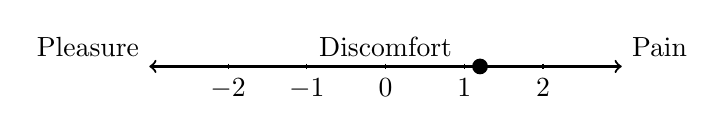
\begin{tikzpicture}
		\draw[thick] (0,1) -- (0,1) node[anchor=south]{Discomfort};
		\draw[thick,->] (0,1) -- (-3,1) node[anchor=south east]{Pleasure};
		\draw[thick,->] (0,1) -- (3,1) node[anchor=south west]{Pain};
		\foreach \x in {-2,-1,0,1,2}
			\draw (\x cm,1pt + 1 cm) -- (\x cm,-1pt + 1 cm) node[anchor=north] {$\x$};
		\fill[black] (1.2, 1) circle (1mm);
	\end{tikzpicture}
	\centering
\end{figure}


A scale of attributed pleasure value $\rho$ integrated over the time of an activity can be defined as the sum of the integrated change in pleasure with respect to that activity:
\begin{equation}\label{phidef}
	\varphi = \int{ \Delta \rho  \:  dt }
\end{equation}





\subsection{Individual trade-off}
An individual will (generally) opt to choose the option at any time that is has the most $\varphi$, such as doing option $a$ or not doing option $a$. When ignoring time delay factors a trade for $a$ can be expressed as:
\begin{equation}\label{ind_trd}
	\varphi_{option} > \varphi_{alternative}
\end{equation}
However when time difference is relevant, the pleasure and pain become subject to the expected or anticipated $\varphi$. Notice that the factors subject to time also has an effect in relation to the decision to make a trade.
\begin{equation}\label{ind_trd_tm}
	\varphi_{anticipated} + \varphi_{timeSubdugation} > \varphi_{alternative}
\end{equation}


\subsection{Exchanges}
The first assumption that must be made here is that the individual scaling of $\rho$ remain independent from both parties exchanging any form of effort. If person one ($p1$) and person two ($p2$) each \textit{perceive} the exchange as being the higher $\varphi$ it in therefore deemed in each of their own individual interests.
\begin{equation}\label{trade_def}
	(\varphi_{p1, trade} > \varphi_{p1, noTrade}) \cup (\varphi_{p2, trade} > \varphi_{p2, noTrade})
\end{equation}\\
when given options of trades people will choose the option that has the highest increment of $\varphi$
\begin{equation}\label{trade_chc}
	rows
\end{equation}


\subsection{Methodology of Analysis}

\subsection{Trade and Exchange}

\subsection{Time Dependent Problems}

\subsection{Probability Dependent Problems}

\subsection{Examples in Business}

\subsection{Examples in Marketing}
In order for there to be mutual benefit in marketing the exchange hinges on the amount of effort that the customer would have to expend in order to make an informed choice. Even if the information rendered is incorrect it is still a starting point where the customer could more easily confirm or debunk the information. As well as this there are too many options or 'deals' for one person to sort through. You could imagine how high the stack would be if they were all printed out. The effort that would be needed to sort through this pile and evaluate each one with respect to how beneficial it would be while considering the probability of a false claim, not to mention the effort required to self educate in order to interpret the value of a deal so well that they could spot what is not in a deal as well. 

With this perspective in mind the value to the customer that an advertisement has as well as sales people's time can be evaluated in terms of the effort saved by the customer. The effort saved is not relative to the customer doing all the research instead to the next best option that is available to the customer. 

\subsection{Governance and Involuntary Trading}
This section attempts to discuss the effects that non consensual trade (in the context of this paper) that is implicit in the role of government.

\subsection{Ethics}
Perhaps it is appropriate to include a section on the ethics of the types of dynamics at play discusses in these chapters. This is subject to the perspective of the reader as it is not uncommon for people to perceive situations in entirely different terms particularly when terms such as involuntary. However the perspective that this document seeks to put forward can shed some light on ethical conundrums. 

A criticism often levelled at ideologies that favour free trade or in more general terms larger degrees of purely voluntary exchange, is that advertising has a negative effect on the 


\end{document}


word graveyard



made entirely by hand from a manufacturer, expludin the use of tools is the from the perspective of the producer  to provide it to the provider and less 
than that of the next best option to the recipient.

When given the chance people will make voluntary exchanges in order to reduce their total effort output. This 
exchange will be made if the option is of lower net effort than the next best option. 
People tend to arrange all economic activity in turms of effort. 


Efficiently: typically in engineering no system can have an efficiency of more than 1, however in this context the $e$ acts as a coefficient of the $(\delta v output) / ( \delta v input)$. As sometimes storing things can add to the value it is possible to get more pleasure from it than was put in.

That there are only labour costs and nothing else. For example take any product or service, the price is defined as only the total of all labour coast associated with the product. in manufacturing a product is often broken down into labour costs and non-labour costs. Non-lobar costs often include materials, parts, tools, tool ware, tool depreciation and transport costs. I would like to assert that this may be true of the current level of manufacturing but not true when considering all layers of production. from example a product that is the comprised of a raw material and labour can be expressed as the sum of the labour of that processes as well as the labour involved in extracting and transporting the raw material. 

All claims made with respect to trading assume a free market.



The only instance where mutual benifit is not met is wjen government interfears    



at a fundamental level human interaction can be ranked on a scale of pleasure and pain. Henceforth denoted as $\rho$. This can be used to describe the pleasure of an event at an instant in time. similar to the concept of black body radiation the idea of there being a value of $\rho$ is absolute and is the identical scale between people. What does not remain constant is that two people may have two values of $\rho$ for the same activity as it's level of effect varies subjectively \\
\begin{figure}[!h]
	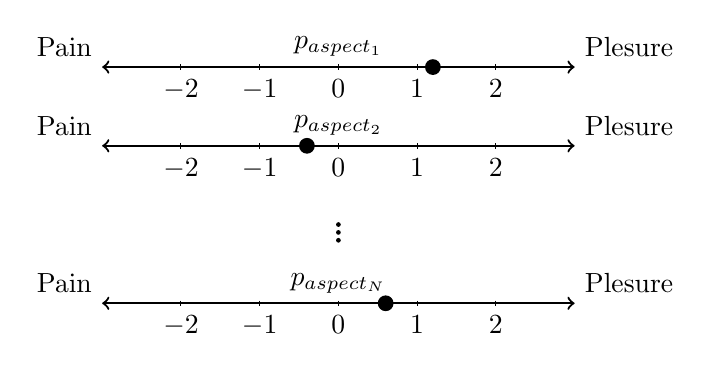
\begin{tikzpicture}
		\draw[thick] (0,1) -- (0,1) node[anchor=south]{$p_{aspect_{1}}$};
		\draw[thick,->] (0,1) -- (-3,1) node[anchor=south east]{Pain};
		\draw[thick,->] (0,1) -- (3,1) node[anchor=south west]{Plesure};
		\foreach \x in {-2,-1,0,1,2}
			\draw (\x cm,1pt + 1 cm) -- (\x cm,-1pt + 1 cm) node[anchor=north] {$\x$};
		\fill[black] (1.2, 1) circle (1mm);
		
		\draw[thick] (0,0) -- (0,0) node[anchor=south]{$p_{aspect_{2}}$};
		\draw[thick,->] (0,0) -- (-3,0) node[anchor=south east]{Pain};
		\draw[thick,->] (0,0) -- (3,0) node[anchor=south west]{Plesure};
		\foreach \x in {-2,-1,0,1,2}
			\draw (\x cm,1pt) -- (\x cm,-1pt) node[anchor=north] {$\x$};
		\fill[black] (-0.4,0) circle (1mm);
		
		\foreach \x in { 0, -0.1, -0.2}
			\fill[black] (0, \x - 1) circle (0.3mm);
			
		\draw[thick] (0,-2) -- (0,-2) node[anchor=south]{$p_{aspect_{N}}$};
		\draw[thick,->] (0,-2) -- (-3,-2) node[anchor=south east]{Pain};
		\draw[thick,->] (0,-2) -- (3,-2) node[anchor=south west]{Plesure};
		\foreach \x in {-2,-1,0,1,2}
			\draw (\x cm,1pt -2 cm) -- (\x cm,-1pt -2 cm) node[anchor=north] {$\x$};
	\fill[black] (0.6, -2) circle (1mm);
	\end{tikzpicture}
	\centering
\end{figure}
\\


The total of all pleasure and pain that an individual is experiencing at any one time is $P$ where:
\begin{equation}\label{Pdef}
	P = \sum \rho
\end{equation}


This can be thought of as a fundamental store input of value. Not necessarily the output of value ether. Since the exact scale of value for each individual is not represented in a standardised format translatable to another The effective of 'value' ($\varphi$). An efficient can only be meaningful in the context of the individual's 'value' spent to that of the potential 'value' returned.
\begin{equation}
	\eta = \frac{\varphi_{potentualOutput}}{\varphi_{input}} 
\end{equation} 
This value is not limited to the traditional domain of $\left\lceil 0, 1 \right\rceil $, instead being capable of residing at $>1$.



The distinction between the local coordinate $p$ and the global coordinate $P$ can be made by overlaying the scales of each individual definition of $p$ to the global scale for an activity. 



that relative value $\varphi$ can be defined numerically as the integral of  potential $p$ over time. where negative numbers represented discomfort two distinctions can be made. first that there is the $\varphi$' that is apparent from the amount of value that has gone into an activity. the second, the amount of value that has been saved by acquiring 'v' value. 'delta



the range of this scales $\left\lceil - \infty, \infty \right\rceil $. Where activities can have a $p$ value that changes over time. Due to how humans perceive meaning moralistically, an arbitrary scale can be assignment to this dimension as the most meaningful or pleasurable things will 'resize' the scale
